\documentclass[a4paper, 12pt]{extreport}
\usepackage[margin=1in]{geometry}
\usepackage{tikz}
\usepackage{setspace}
\graphicspath{ {../../resources/images/} }
\usepackage[titles]{tocloft}
\usepackage{titlesec}
\usepackage[hidelinks]{hyperref}
\usepackage{pdfpages}
\titleformat{\chapter}[hang]{\huge\bfseries}{\thechapter}{20pt}{\vspace{0.5em}}
\titlespacing*{\chapter}{0pt}{-3em}{1.1\parskip}
\usepackage[backend=biber, style=ieee]{biblatex}
\usepackage{parskip}
\setlength{\parindent}{1cm}
\setlength{\parskip}{.5\baselineskip}
\usepackage[nottoc,numbib]{tocbibind}
\addbibresource{../../resources/citation.bib}

\begin{document}

	\onehalfspacing
	
	\begin{titlepage}
		
		\begin{tikzpicture}[remember picture, overlay]
			\node[xshift=14cm,yshift=-1.8cm,anchor=north west] at (current page.north west){%
				
\includegraphics[height=2.5cm]{logos/sunway}};
		\end{tikzpicture}
		
		\vfill
		
		\begin{center}
			\textbf{\large CAPSTONE PROJECT 1} \\
			\textbf{\large Planning Document} \\
			\vspace{1cm}
			\textbf{\large Evaluation of Nature-inspired Optimisation\\Algorithms in Solving Versus Tetris}
			
			\vspace{1cm}
			
			by
			
			\vspace{1cm}
			
			\large Yap Wei Xiang \\
			21067939
			
			\vspace{1cm}
			
			\large Supervisor: Dr Richard Wong Teck Ken
			
			\vspace{1cm}
			
			\normalsize Semester: April 2024 \\
			Date: % DATE OF SUBMISSION
			
			\vfill
			
			Department of Computing and Information Systems\\
			School of Engineering and Technology\\
			Sunway University
		\end{center}
		
	\end{titlepage}
	
	\pagenumbering{roman} % switch to roman numerals
	
	\chapter*{Abstract}
	
	\addcontentsline{toc}{chapter}{Abstract}
	
	\tableofcontents
	
	\chapter{Introduction}
	
		\pagenumbering{arabic}
		
		% What is Tetris		
		Tetris is a popular video game created in 1984 by computer programmer Alexey Pajitnov  \cite{about-tetris}. It is a puzzle game that requires players to strategically place sequences of pieces known as "Tetriminos" into a rectangular Matrix (refer to Figure \ref{tetrisgame}). In the classic game, players attempt to clear as many lines as possible by completely filling horizontal rows of blocks, but if the Tetriminos surpass the top of the Matrix, the game ends.
		
		\begin{figure}[h]
			\centering
			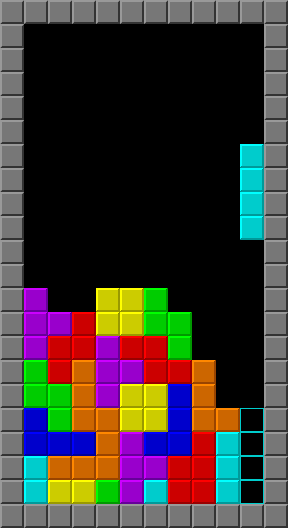
\includegraphics[scale=0.5]{/cp1/typical_tetris_game}
			\caption{A Typical Tetris Game}
			\label{tetrisgame}
		\end{figure}
		
		% Tetris and computer science
		Since its release, mathematicians and computer scientists have been intrigued by the game of Tetris, leading to a diverse array of research endeavours exploring the various facets of the game, including its computational complexity \cite{tetris-is-hard-even-to-approx}, and its possibility of being won \cite{can-you-win-at-tetris} \cite{how-to-lose-at-tetris}.
		
		\section{Motivation}
		
			% In this section, you'll explain why your capstone project is important and relevant. What inspired you to pursue this topic? Is there a particular problem or challenge in the field that you're interested in addressing?
			% Consider discussing the broader significance of your research topic, such as its potential impact on society, industry, or academia. Why should readers care about your project?
			% You might also highlight any personal or professional experiences that motivated your interest in the topic.
	 		
	 		In their paper, \citeauthor{tetris-is-hard-even-to-approx} showed that it is NP-complete to optimise several natural objective functions of Tetris \cite{tetris-is-hard-even-to-approx}. NP-completeness poses a significant challenge in computational problem-solving, as it denotes the absence of polynomial-time algorithms for efficient solutions \cite{npcomplete}. Moreover, the discovery of a polynomial-time algorithm for any NP-complete problem implies that any problem in the set of NP, encompassing efficiently verifiable but potentially difficult problems, could be solved in polynomial time \cite{npcomplete}. NP-completeness extends beyond Tetris, with real-life instances of NP-complete arising in diverse fields such as route optimisation \cite{route-optimisation-np-complete}, job scheduling \cite{job-scheduling-np-complete}, medicine \cite{medical-diagnosis-np-complete} and more.
	 		
	 		To address these challenges, researches have explored alternative approaches to tackle NP-complete problems, including the use of as nature-inspired algorithms \cite{job-shop-ga}. Although they might fail at finding optimal solutions, nature-inspired algorithms are able to return acceptable solutions in shorter running times \cite{review-nia-wael}. In the context of optimising Tetris gameplay, studies have shown the effectiveness of using nature-inspired algorithms in playing the classic single-player game \cite{tetris-ga-lewis} \cite{swarm-tetris}. However, there remains limited research on the effectiveness of nature-inspired optimization algorithms in the multiplayer versus variant of the game.
			
		\section{Problem Statement}
			
			% Here, you'll clearly define the problem or issue that your capstone project aims to address. What specific challenge or question are you seeking to answer?
			% Describe the current state of the problem and any existing solutions or approaches. What limitations or shortcomings do these solutions have?
			% Be concise and specific in articulating the problem statement, making it clear to readers what your project seeks to contribute to the field.
			
			% Despite the extensive research on classic Tetris, there is a significant gap in the literature regarding its multiplayer versus variant (refer to Figure \ref{tetrio}). This gap presents an intriguing problem within the field of computational gaming, as understanding the optimal strategies, challenges, and computational complexities unique to multiplayer versus Tetris remains largely uncharted territory.
			
			\textit{Versus Tetris} (refer to Figure \ref{tetrio}) presents a unique challenge in computational gaming due to its complex dynamics and real-time competitive nature. While previous research regarding the use of nature-inspired algorithms for Tetris optimisation have focused on single-player scenarios, the effectiveness of these algorithms in the multiplayer context remains largely unexplored. Despite the demonstrated success of these algorithms in improving single-player Tetris gameplay, their application to the multiplayer variant poses distinct challenges due to a novel rule set and differing objectives that require further investigation.
			
			\begin{figure}
				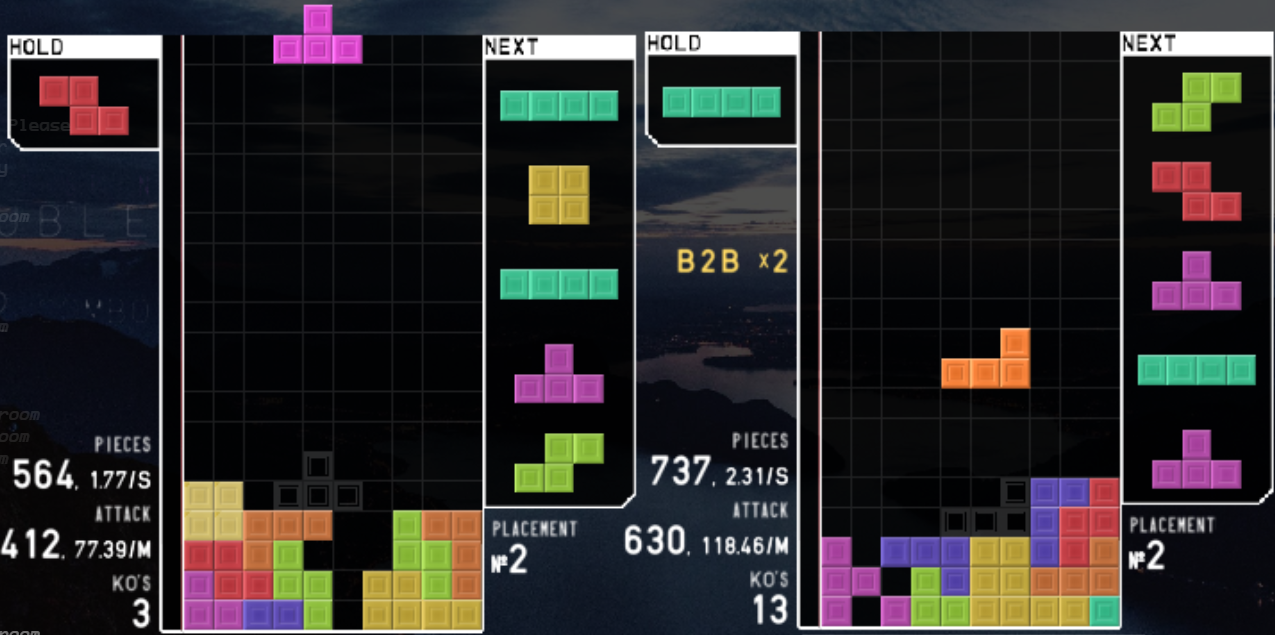
\includegraphics[width=\textwidth]{/cp1/tetrio}
				\caption{A Screenshot of a Game of Tetr.io, a Fan-made Versus Tetris Game}
				\label{tetrio}
			\end{figure}
		
		\section{Aim}
		
			% The aim of your project is its overarching goal or objective. What do you hope to achieve through your research?
			% Summarize the main purpose of your project in a single sentence or paragraph. This should provide a clear, concise statement of what you intend to accomplish.
			% Your aim should align closely with the problem statement and reflect the broader motivation for your research.
			
			The aim of this capstone project is to evaluate the viability of nature-inspired optimisation algorithms in solving the game of Versus Tetris. By integrating insights from nature-inspired algorithms, the project seeks to create a robust and adaptable Tetris-playing software capable of competing against human players or other Tetris-playing programs. Through this endeavour, the project aims to contribute valuable insights into the application of nature-inspired algorithms in addressing complex gaming environments and advancing the field of computational gaming.
		
		\section{Objectives}
		
			% Objectives are specific, measurable outcomes that you aim to achieve in order to fulfill your project's aim.
			% List the key objectives of your project, breaking them down into actionable steps or milestones. These objectives should directly address the problem statement and contribute to achieving the project's aim.
			% Consider using the SMART criteria (Specific, Measurable, Achievable, Relevant, Time-bound) to ensure that your objectives are well-defined and achievable within the scope of your project.
			
			The objectives of this project are as follows:
			
			\begin{enumerate}
				\item Formulate the problem of Versus Tetris for game AI.
				\item Research and implement a variety of nature-inspired optimisation algorithms to determine their suitability for optimising gameplay strategies in Versus Tetris.
				\item Design a comprehensive framework for objectively evaluating and comparing the performance of the algorithms.
				\item Develop a playable game of Tetris that simulates gameplay and training.
				\item Using the game, do comparative analyses with the designed framework to assess the effectiveness and efficiency of each algorithms.
				\item Summarize findings from the comparative analyses, highlighting the strengths and weaknesses of each nature-inspired optimisation algorithm.
			\end{enumerate}
		
		\section{Project Scope}
			
			% Define the boundaries and focus areas of your capstone project in terms of its scope. What aspects of the problem will you address, and what will you exclude?
			% Discuss any limitations or constraints that may impact the scope of your project, such as time, resources, or access to data.
			% Clarify what readers can expect to find within the scope of your project and what may fall outside its boundaries.
			
			This project will focus specifically on the evaluation of nature-inspired optimisation algorithms in the context of multiplayer versus Tetris. It will entail the development of a playable Tetris game capable of simulating gameplay and the training of algorithms. This simulation environment will facilitate in the analysis and evaluation of these algorithms' performances. The scope includes the exploring of a range of nature-inspired algorithms to address the unique challenges inherent in Versus Tetris.
			
		
		% Exceptional overview of the proposed project.
		% The problem statement, objectives, scope of work, methodology, proposed outcome and timeline are written in a clear precise manner and presented in proper order.
	
	\chapter{Literature Review}
		
		% A well-articulated introduction that provides a clear, logical, and succinct description of content, scope, and organization of the review which draws the reader's attention to a central concern, debate or contention.
		% Body of section includes citations to a range of reliable sources that critically substantiate and contextualizes all major claims made.
		% Exceptional discussion that summarizes the body of review, highlights the most important findings (in your opinion) and its implication to the direction of the project.
		% Section is very well organized.
		% The review has clarity, simplicity, parsimony, which includes clear transitions and systematic use of headings and subheadings.
		
		% wtf is np-complete
		% 
		
		\section{What is Versus Tetris?}
	
	\chapter{Technical Plan}
	
		% Graphical and textual description is provided for flow of information between components in the system/stages in the research study.
		% Graphical overview of system/research study corresponds to the textual description provided with no errors.	
		%Excellent description is provided for all methodologies, tools and techniques used to specify, design, build, test, integrate, document and deliver work products throughout the project along with the relevant supporting documents.
		% All documents provided are well-drawn/well-written, complete and correct. The purpose and role of each document in the project is stated clearly.
	
	\chapter{Work Plan}
		
		% Excellent description of all work activities to be performed during the project, relationship among the activities and the resultant work products for each activity.
		% Scheduled duration for each work activity is justified and supported by the identified project risk factors and work decomposition that each activity requires.
		% The whole project schedule, milestones and activitiy lists are depicted professionally on the Gantt chart with all dependencies, predecessor and successor work activities denoted clearly.
	
	\printbibliography[heading={bibnumbered}, title={References}]
		
\end{document}